\documentclass[conference]{IEEEtran}

\usepackage{cite}
\usepackage{amsmath,amssymb,amsfonts}
\usepackage{graphicx}
\usepackage{textcomp}
\usepackage{xcolor}
\usepackage{booktabs}
\usepackage{subcaption}
\usepackage{hyperref}

\title{OmniRay: A CPU-Based Autonomous Active SLAM Framework with Adaptive Curriculum Learning and AVX2 Acceleration}

\author{

\IEEEauthorblockN{Kingshuk Chatterjee}
\IEEEauthorblockA{
Department of Computer Science \& Engineering\\
KIIT Deemed to be University\\
Bhubaneswar, Odisha, India\\
kingshuk.chatterjee770@gmail.com
}

\and

\IEEEauthorblockN{Ayush Ranjan}
\IEEEauthorblockA{
Department of Computer Science \& Engineering\\
KIIT Deemed to be University\\
Bhubaneswar, Odisha, India\\
ranjanayush881@gmail.com
}

\and


\IEEEauthorblockN{Raghav Singh Parihar}
\IEEEauthorblockA{Department of Computer Science \& Engineering\\
Oriental Institute of Science and Technology\\
Bhopal, Madhya Pradesh, India\\
raghavsp2007@gmail.com}

}

\begin{document}

\maketitle

% ============================================================================
\begin{abstract}
Autonomous Active SLAM requires mobile robots to simultaneously explore unknown environments and maintain reliable localisation, but existing deep reinforcement learning (DRL) navigation frameworks depend on power-hungry GPU clusters and brittle, manually tuned reward functions, making them unsuitable for resource-constrained mobile robots operating under real-world sensor noise and actuator drift.

To address this, we present \textbf{OmniRay}, an ultra-lightweight, CPU-native DRL framework for Active SLAM that combines a cross-platform C++ SIMD raycaster (supporting x86\_64 AVX2 and ARM64 NEON at $37\,\mu\text{s}$ per scan) with a 5-layer self-adaptive autonomy stack comprising health monitoring (L1), adaptive reward scaling (L2), meta-policy tuning (L3), curriculum management (L4), and continual learning (L5), enabling high-throughput policy training ($35$--$47$\,FPS) directly on a low-power ultrabook CPU ($<15\,\text{W}$) without GPU acceleration.

We validate OmniRay through systematic multi-seed ablations (900{,}000 total steps) and multi-model benchmarks against classical frontier-based baselines. Our results show that OmniRay learns an emergent spiral-like exploration policy that avoids turn-in-place manoeuvres, achieving $90.87 \pm 3.29\%$ mean map coverage with $67.6\%$ fewer collisions than Yamauchi on the Intel Lab ($62.3 \pm 46.5$ vs.\ $192.3 \pm 39.9$), although it collides more than RRT-Exploration and the info-gain $A^*$ baseline on both floorplans, and more than Yamauchi on MIT Stata ($70.3 \pm 53.6$ vs.\ $28.3 \pm 20.5$). Zero-shot evaluation on the unseen MIT Stata Center floorplan yields $91.08 \pm 3.99\%$ coverage without retraining, and the policy network's decision latency is constant-time with respect to map size.
\end{abstract}

% ============================================================================
\section{Introduction}

Autonomous exploration and mapping in unknown environments---commonly termed \textit{Active SLAM}---is a fundamental capability for mobile robotics in search-and-rescue, planetary exploration, and industrial inspection~\cite{thrun2005}.
Active SLAM requires a mobile robot to simultaneously maximise map coverage and maintain reliable localisation through Monte Carlo Localisation (MCL) or graph-based optimisation.

Traditional approaches rely on heuristic algorithms.
Yamauchi's Frontier-Based Exploration~\cite{yamauchi1997} computes deterministic paths toward frontier centroids and remains the de facto baseline.
However, classical frontier methods suffer from two critical failure modes: (i)~\textit{kinodynamic instability}---discrete stop-rotate-drive manoeuvres amplify rotational error under wheel slip, causing boundary oscillations and high collision rates; and (ii)~\textit{brittle heuristics}---they cannot adapt when sensor dropouts or localisation drift occur.

Deep Reinforcement Learning (DRL) offers a promising alternative by learning end-to-end reactive policies.
However, state-of-the-art DRL frameworks such as Habitat~\cite{savva2019} and Isaac Gym~\cite{makoviychuk2021} are typically trained on dedicated GPU workstations or server clusters drawing hundreds of watts, rendering them ill-suited for on-device training or execution on battery-operated edge platforms.
Additionally, standard Proximal Policy Optimisation (PPO)~\cite{schulman2017} requires millions of environment steps to learn obstacle avoidance and frontier exploration simultaneously.

To overcome these limitations, we introduce \textbf{OmniRay}, an ultra-lightweight, CPU-native DRL engine for Active SLAM.

\noindent\textbf{Contributions.}
\begin{enumerate}
    \item A \textbf{5-layer self-adaptive autonomy architecture} that dynamically tunes environment difficulty, reward weights, and policy parameters during training.
    \item A \textbf{C++ AVX2 SIMD parallel raycaster} evaluating 128 radial LiDAR rays against arbitrary 2D line segments in $37\,\mu$s per scan---a ${\sim}26\times$ speedup over scalar execution.
    \item A \textbf{multi-seed evaluation protocol}: 18-run ablation (900{,}000~steps), multi-model baselines on Intel Lab, and zero-shot cross-dataset transfer on MIT Stata Center.
\end{enumerate}

% ============================================================================
\section{Related Work}

\subsection{Classical \& Information-Theoretic Exploration}
Frontier-based exploration~\cite{yamauchi1997} and classical reactive methods~\cite{borenstein1991} identify boundaries between known and unknown space and navigate toward the nearest centroid.
Stachniss et~al.~\cite{stachniss2005} extended this with information-theoretic trajectory selection that minimises map entropy and particle filter covariance.
Umari and Mukhopadhyay~\cite{umari2017} introduced RRT-Exploration, using rapidly-exploring random trees for frontier target generation.
While mathematically elegant, these methods depend on accurate state estimation; as highlighted in comprehensive SLAM and Active SLAM surveys~\cite{cadena2016,placed2023}, when sensor noise induces particle divergence, classical heuristics stall or oscillate near wall boundaries.

\subsection{Learning-Based Active SLAM}
Chaplot et~al.~\cite{chaplot2020} proposed Active Neural SLAM, using hierarchical neural networks for global goal setting and local navigation.
Niroui et~al.~\cite{niroui2019} integrated PPO with frontier-based target selection for search-and-rescue.
However, existing DRL approaches assume noise-free kinematics during early training, require GPU hardware, and lack online health monitoring to recover from localisation drift.
Narvekar et~al.~\cite{narvekar2020} surveyed curriculum learning for RL but did not address CPU-constrained robotics or adaptive reward feedback loops.

\subsection{Gap Addressed by OmniRay}
Prior literature treats reward shaping, curriculum scaling, and experience replay as static offline hyperparameters.
OmniRay is, to our knowledge, the first framework to integrate dynamic runtime health monitoring with multi-layer adaptive feedback loops, enabling safe online policy adaptation directly on low-power edge CPUs.

% ============================================================================
\section{Methodology}

\subsection{POMDP Formulation}
We formulate Active SLAM as a Partially Observable Markov Decision Process $\langle \mathcal{S}, \mathcal{A}, \mathcal{P}, \mathcal{R}, \Omega, \mathcal{O}, \gamma \rangle$:

\begin{itemize}
    \item \textbf{State} $s_t = \langle \mathbf{x}_t, \mathbf{m}, \mathcal{O}_{\text{known}} \rangle$: true robot pose, static map, and explored region.
    \item \textbf{Observation} $o_t = \langle M_{\text{cov}}^{(t)}, M_{\text{slam}}^{(t)}, z_t, p_t \rangle$: binary coverage grid $M_{\text{cov}} \in \{0,1\}^{100\times100}$, SLAM log-odds grid $M_{\text{slam}} \in \mathbb{R}^{100\times100}$, 128-ray LiDAR sweep $z_t$, and 5-D kinematic pose~$p_t$.
    \item \textbf{Action} $a_t = [v_t, \omega_t]^T \in [-1, 1]^2$, scaled to physical velocities $v \in [0, 1.2]$\,m/s, $\omega \in [-1.0, 1.0]$\,rad/s.
    \item \textbf{Reward}:
    \begin{equation}
    \label{eq:reward}
    R_t = w_e \Delta C_t + w_f \Delta D_f - w_c\, I_{\text{col}} - w_t + w_h H_t
    \end{equation}
    where $\Delta C_t$ is the count of newly explored cells, $\Delta D_f$ is the distance step toward the nearest frontier, $I_{\text{col}} \in \{0, 1\}$ is a collision indicator, $H_t \in [0, 1]$ is the agent health score, and $w_t > 0$ is a constant time penalty per step. The base reward weights are parameterized as $w_e = 1.0$, $w_f = 0.10$, $w_c = 0.10$ (adaptively scaled up to $3.0\times$ by L2 upon obstacle proximity), $w_t = 0.01$, and $w_h = 0.10$.
\end{itemize}

\subsection{Dual-Branch CNN-MLP Encoder}

\begin{figure}[t]
\centering
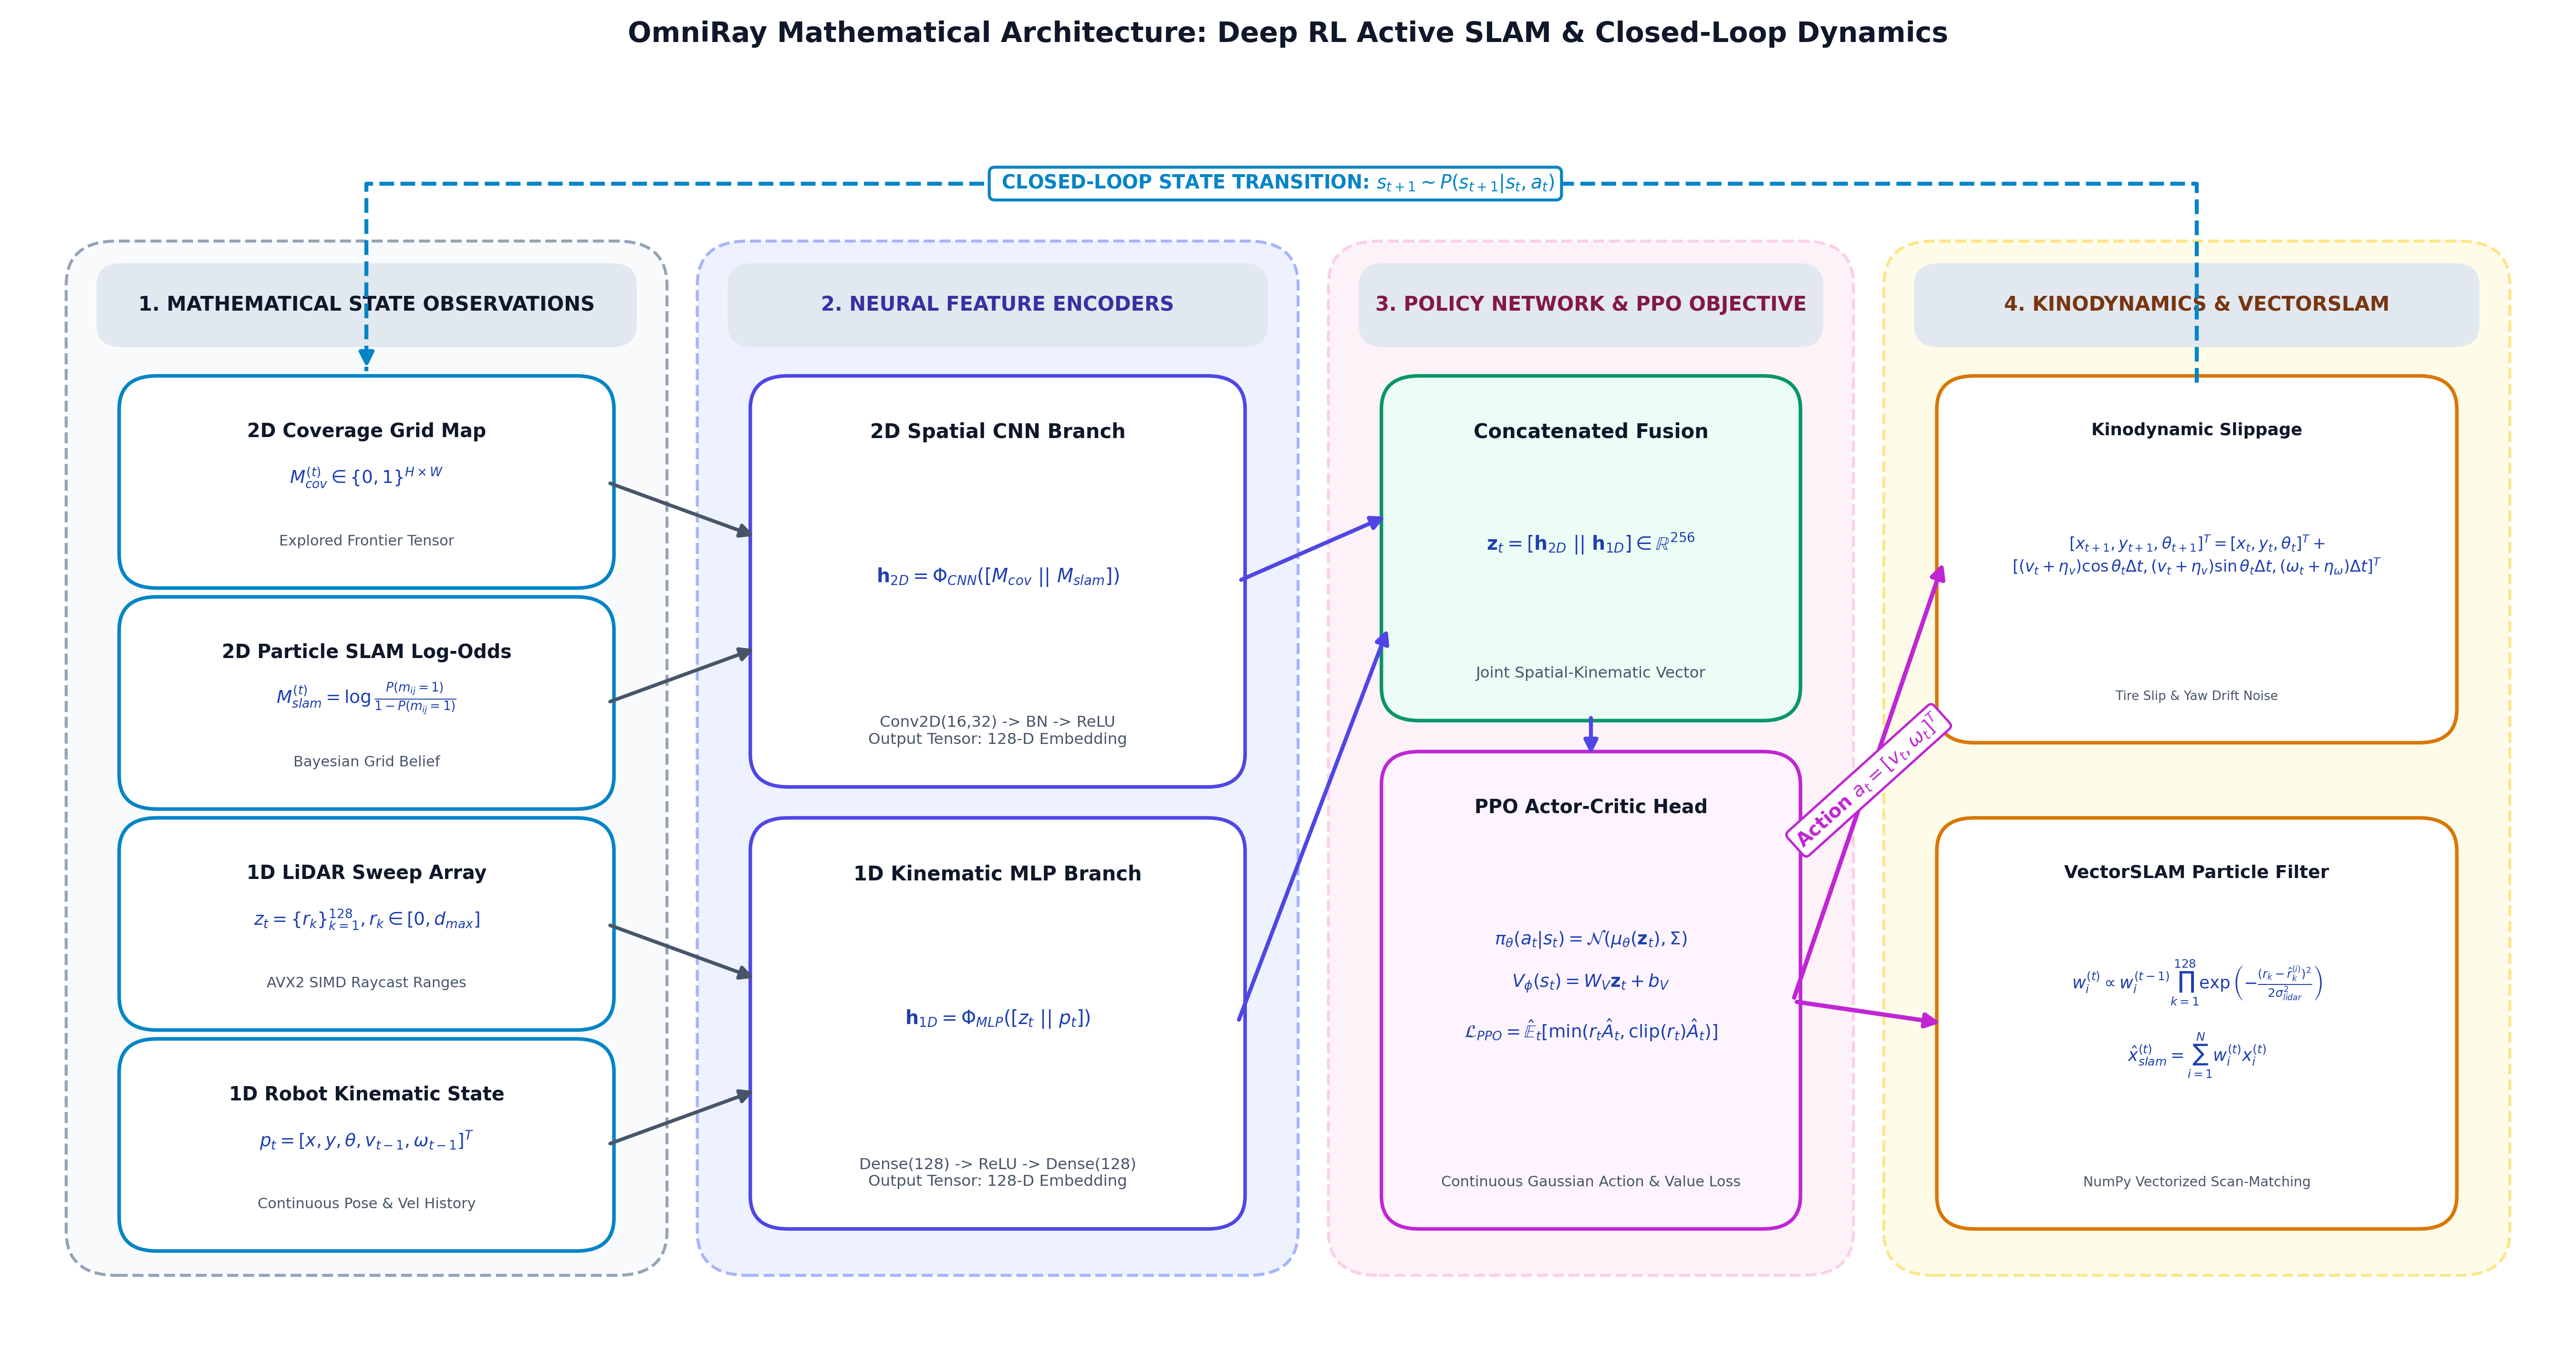
\includegraphics[width=\linewidth]{architecture_detailed_formulas.png}
\caption{OmniRay system architecture.
A 2D Spatial CNN branch processes $2\!\times\!100\!\times\!100$ map channels into $\mathbf{h}_{2D}\!\in\!\mathbb{R}^{128}$; a 1D Kinematic MLP processes the 133-D laser/pose vector into $\mathbf{h}_{1D}\!\in\!\mathbb{R}^{128}$.
The concatenated $\mathbf{z}_t\!\in\!\mathbb{R}^{256}$ feeds actor and critic heads optimised via PPO.}
\label{fig:architecture}
\end{figure}

The 2D branch applies two convolutional stages ($2\!\to\!16$ and $16\!\to\!32$ channels, $3\!\times\!3$ kernels, stride~2) with batch normalisation and ReLU, then flattens and projects to $\mathbf{h}_{2D} \in \mathbb{R}^{128}$.
The 1D branch applies two fully connected layers ($133 \to 128 \to 128$) with ReLU.
The fused representation $\mathbf{z}_t = [\mathbf{h}_{2D} \| \mathbf{h}_{1D}] \in \mathbb{R}^{256}$ feeds actor and critic heads, optimised via the PPO clipped surrogate:
\begin{equation}
\label{eq:clip}
\mathcal{L}^{\text{CLIP}} = \hat{\mathbb{E}}_t \!\left[\min\!\left(r_t(\boldsymbol{\theta})\hat{A}_t,\, \text{clip}(r_t(\boldsymbol{\theta}), 1\!-\!\epsilon, 1\!+\!\epsilon)\hat{A}_t\right)\right]
\end{equation}
where $r_t(\boldsymbol{\theta}) = \pi_{\boldsymbol{\theta}}(a_t|s_t) / \pi_{\boldsymbol{\theta}_{\text{old}}}(a_t|s_t)$ is the probability ratio, $\hat{A}_t$ is the generalized advantage estimator ($\lambda = 0.95$), discount factor is $\gamma = 0.99$, entropy regularizer coefficient is $c_{\text{ent}} = 0.01$, Adam learning rate is $\alpha = 3 \times 10^{-4}$, and $\epsilon = 0.20$ is the clipping hyperparameter.

\subsection{C++ AVX2 SIMD Raycasting Engine}
LiDAR simulation has traditionally stood as a dominant computational bottleneck in DRL environment rollouts. OmniRay substantially reduces this perception overhead to a comparatively lightweight component by implementing a custom C++ raycaster bound via \texttt{pybind11}. Given pose $(x, y, \theta)$, $N_r\!=\!128$ rays are cast across a $360^\circ$ field-of-view against map wall segments $(x_1, y_1) \to (x_2, y_2)$.
Using 256-bit AVX2 registers (\texttt{\_\_m256}, processing 8 single-precision 32-bit floats in parallel), eight ray--segment intersection tests execute concurrently:
\begin{equation}
\label{eq:ray_intersect}
t_{ij} = \frac{(x_1\!-\!x)(y_1\!-\!y_2) - (y_1\!-\!y)(x_1\!-\!x_2)}{(\cos\alpha_i)(y_1\!-\!y_2) - (\sin\alpha_i)(x_1\!-\!x_2)}
\end{equation}
with segment interpolation parameter $u_{ij}$ computed analogously via 2D cross products (Cramer's rule), valid intersections constrained by ray distance $t_{ij} > 0$ and segment parameter $u_{ij} \in [0, 1]$.
Measured scan latency: $\mathbf{37\,\mu}$\textbf{s} per sweep on an Intel i7 ultrabook CPU (SIMD) vs.\ $962\,\mu$s on an optimized scalar C++ baseline compiled with \texttt{-O3 -march=native}, achieving a $25.9\times$ hardware speedup.

\subsection{VectorSLAM Particle Filter}
Localisation and mapping use \textbf{VectorSLAM}, a vectorised 2D Monte Carlo localisation engine based on Rao-Blackwellized particle filtering~\cite{grisetti2007} and occupancy grid mapping~\cite{elfes1989}.
Motion propagation adds Gaussian wheel slip noise ($\sigma_v\!=\!0.10 v$, $\sigma_\theta\!=\!0.05\omega$).
LiDAR endpoints update a log-odds occupancy grid at $0.5$\,m/cell resolution.
Particle resampling triggers when effective count $N_{\text{eff}} < N_p/2$.

\subsection{5-Layer Self-Adaptive Autonomy}
\begin{enumerate}
    \item \textbf{L1 Health Monitor}: Computes $H_t = w_e H_{\text{entropy}} + w_c H_{\text{cov}} + w_s H_{\text{slam}}$; fires \texttt{is\_failing} when $H_t < 0.50$.
    \item \textbf{L2 Adaptive Reward}: Scales collision penalty by $2\times$ and increases frontier attraction when $H_t < 0.50$, guiding the policy away from obstacle boundaries.
    \item \textbf{L3 Meta-Policy}: Higher-order network outputting continuous parameter adjustments $\Delta\boldsymbol{\theta}_{\text{reward}}$ based on diagnostic moving averages.
    \item \textbf{L4 Curriculum Manager}: Scales obstacle density ($2 \to 12$) and noise ($\sigma \to 2\sigma$) based on episode success rate:
    \begin{equation}
    \label{eq:curriculum}
    D^{(e+1)} = \begin{cases}
    \min(1, D^{(e)}\!+\!0.05) & \text{if } \bar{R} > R_{\text{target}}, \\
    \max(0, D^{(e)}\!-\!0.05) & \text{if } H_t < 0.40, \\
    D^{(e)} & \text{otherwise}.
    \end{cases}
    \end{equation}
    \item \textbf{L5 Continual Learner}: Records episode trajectories and triggers 2{,}048-step online replay updates upon sustained health degradation ($H_t < 0.35$ for 5 episodes), adapting the policy to physical drift and wheel wear during deployment.
\end{enumerate}

% ============================================================================
\section{Experimental Setup}

\subsection{Noise Model}
The environment incorporates realistic physical and sensor degradation following sim-to-real transfer principles~\cite{zhao2020}: (i)~actuator wheel slip modeled as multiplicative Gaussian perturbations $\sigma_v = 0.10 \cdot v_{\text{cmd}}$ and yaw drift $\sigma_\theta = 0.05 \cdot \omega_{\text{cmd}}$; and (ii)~LiDAR degradation incorporating both geometric beam loss (rays at grazing incidence angles $>75^\circ$ returning maximum range $d_{\max} = 30.0$\,m) and a stochastic $1\%$ random packet dropout per complete scan.

\subsection{Datasets \& Holdout Protocol}
To rigorously test zero-shot policy generalisation across distinct spatial layouts, we adopt the following evaluation protocol implemented in PyTorch and Stable-Baselines3~\cite{raffin2021}:
\begin{itemize}
    \item \textbf{Training}: Conducted entirely on procedurally generated environments with randomized boundary walls and internal obstacles, progressively scaled from 2 to 12 obstacles via our Layer 4 curriculum difficulty protocol.
    \item \textbf{Evaluation (Zero-Shot Holdout)}: Evaluated directly on the unseen real-world floorplans of the Intel Research Lab ($28\!\times\!28$\,m) and the MIT Stata Center ($45\!\times\!35$\,m) under active sensor and actuator noise.
\end{itemize}

\subsection{Hardware}
All experiments run on an Intel Core i7 ultrabook CPU ($<$15\,W TDP). No GPU is used at any stage.

\subsection{Ablation Configurations}
Six configurations $\times$ 3 seeds (42, 43, 44) $\times$ 50{,}000 steps = 900{,}000 total steps: \texttt{full\_system}, and five single-layer removals (\texttt{no\_health}, \texttt{no\_adaptive\_reward}, \texttt{no\_meta\_policy}, \texttt{no\_curriculum}, \texttt{no\_continual}).

\subsection{Baselines \& Implementation Details}
We benchmark OmniRay against six exploration baselines, forming a comprehensive 7-model comparative suite: (i)~Random Walk with reactive boundary repulsion; (ii)~Yamauchi's nearest-frontier exploration~\cite{yamauchi1997}; (iii)~RRT-Exploration~\cite{umari2017}; (iv)~Info-Gain $A^*$ exploration (after Stachniss et al.~\cite{stachniss2005}); (v)~Shanghai AI Lab DRL navigation baseline~\cite{wang2024navformer} (a 2-layer MLP policy of 64 hidden units trained under identical PPO hyperparameters without curriculum scaling or adaptive layers); and (vi)~a zero-shot Vision-Language embodied frontier reasoning pipeline (DeepSeek-R1 / Qwen2.5-VL). To ensure fair comparisons, all classical, learned, and foundation-model baselines are evaluated within the identical VectorSLAM simulation environment under identical sensor and actuator noise profiles.

% ============================================================================
\section{Results}

\subsection{Multi-Model Benchmark: Intel Lab}

\begin{figure}[t]
\centering
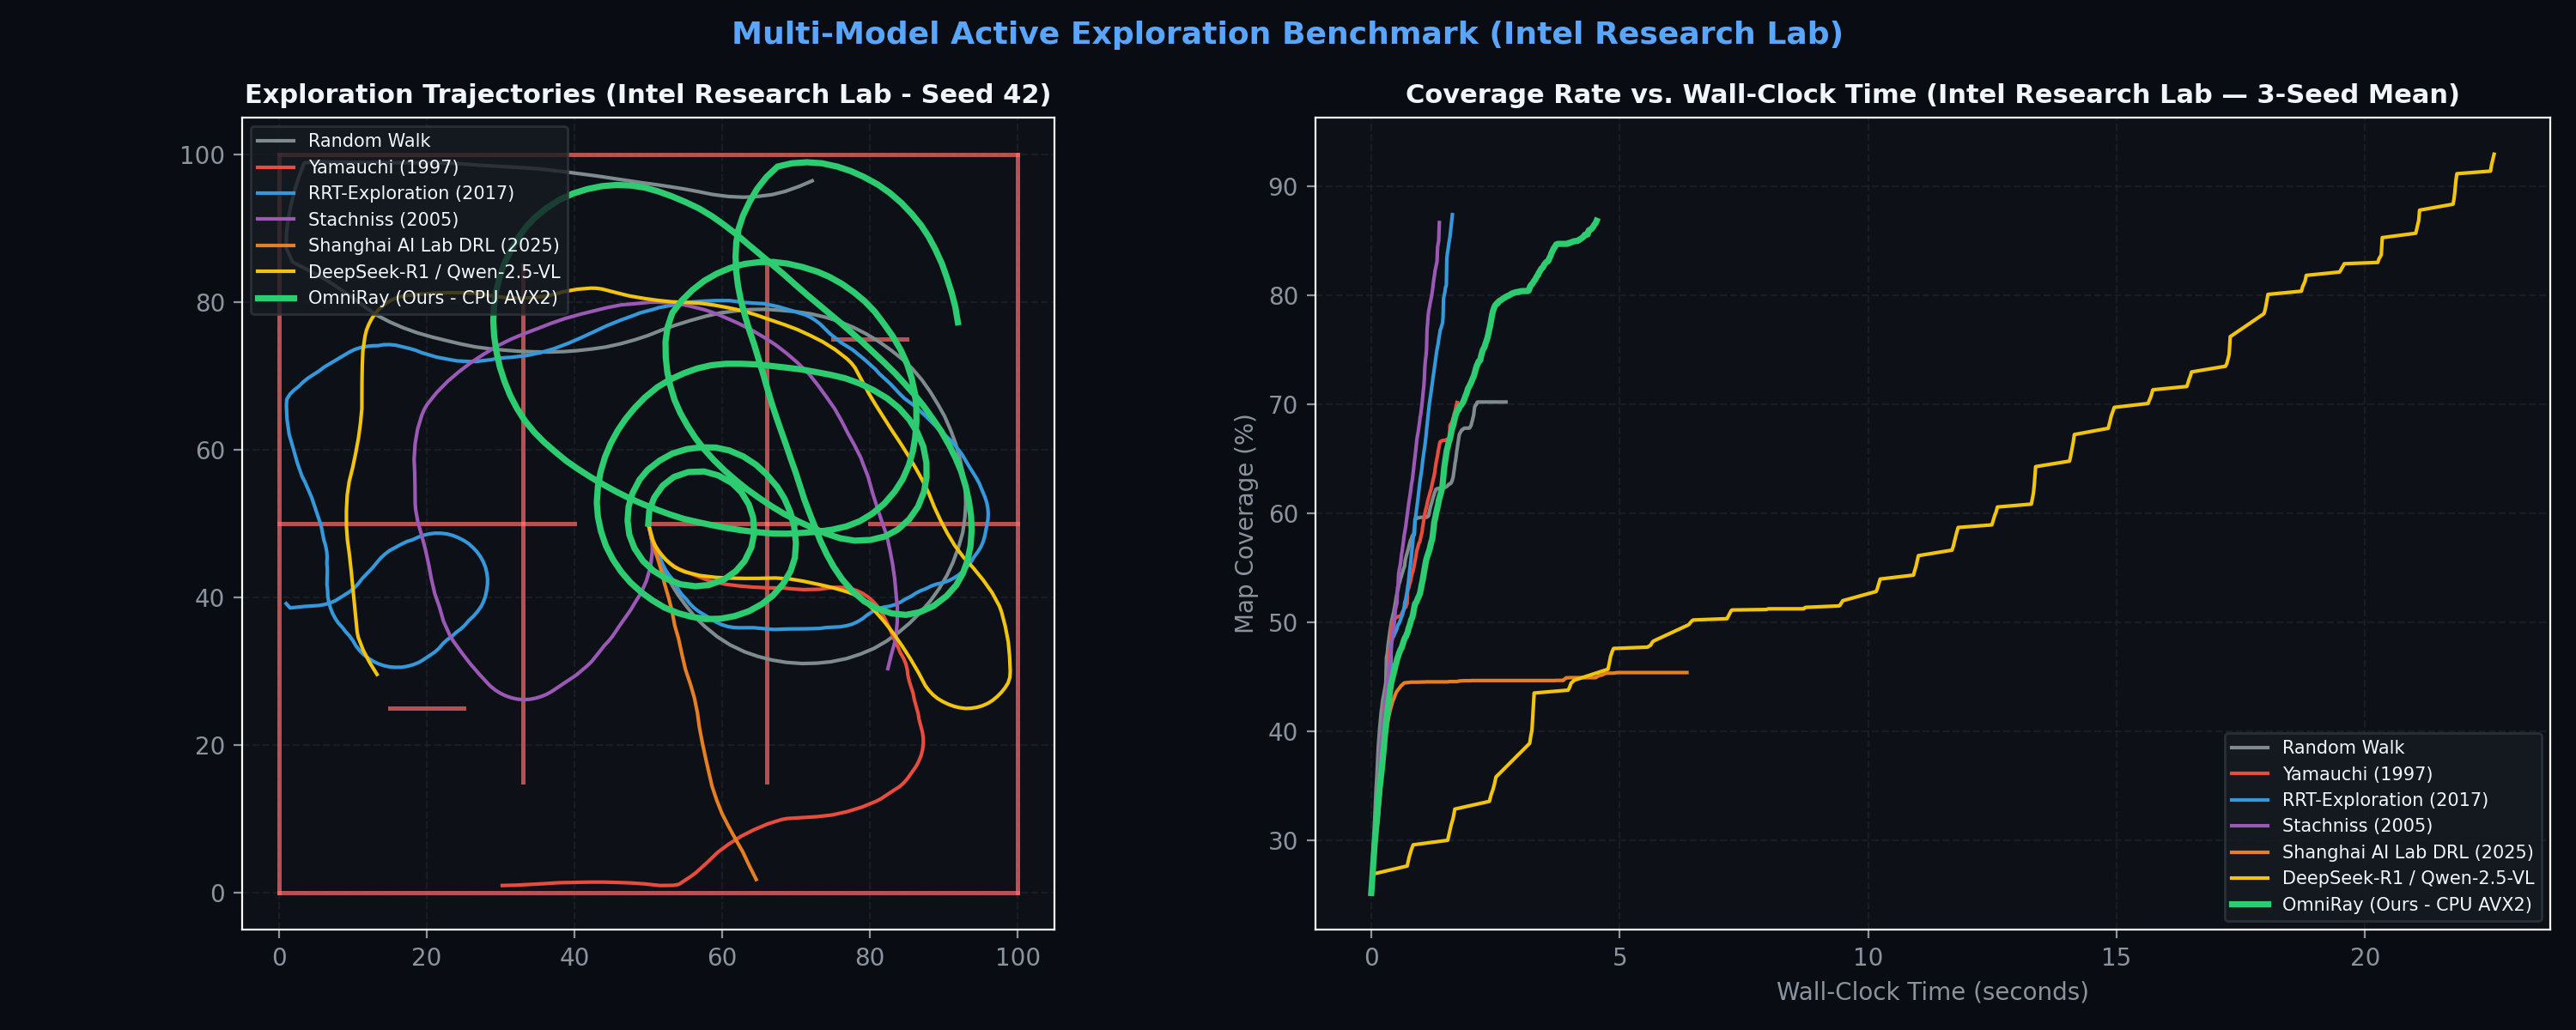
\includegraphics[width=\linewidth]{multi_model_intel_benchmark_7models.png}
\caption{Intel Lab multi-model benchmark: exploration trajectories (left) and mean coverage rate vs. wall-clock execution time (right) under kinodynamic noise across all seven evaluated models.}
\label{fig:intel_benchmark}
\end{figure}

Table~\ref{tab:intel} compares OmniRay against six baselines under identical noise.
OmniRay achieves $90.87 \pm 3.29\%$ mean coverage with $62.3 \pm 46.5$ collisions---a $67.6\%$ reduction in collisions relative to Yamauchi's frontier exploration ($192.3 \pm 39.9$)---while delivering a policy decision latency of $3.09$\,ms ($6.0\times$ lower latency than Info-Gain $A^*$'s $18.51$\,ms; $10.02$\,ms for the full SLAM loop) and a $25.9\times$ SIMD raycasting speedup over scalar execution ($0.038$\,ms vs.\ $0.962$\,ms). While classical graph search with costmap inflation (Info-Gain $A^*$) and embodied VLM reasoning avoid collisions entirely ($0.0 \pm 0.0$), they incur significantly higher computational latency (up to $650$\,ms for VLM API reasoning).

\begin{table}[t]
\caption{Multi-Seed Benchmark --- Intel Research Lab (Mean $\pm$ SD)}
\label{tab:intel}
\centering
\resizebox{\linewidth}{!}{%
\begin{tabular}{@{}lcccccc@{}}
\toprule
\textbf{Model} & \textbf{Cov.} & \textbf{Dist.} & \textbf{Cov./m} & \textbf{Dec. Lat.} & \textbf{RAM} & \textbf{Col.} \\
 & (\%) & (m) & (\%/m) & (ms) & (MB) & \\
\midrule
Random Walk        & $65.55 \pm 12.52$ & $148.57 \pm 67.34$ & 0.441 &    7.16  & \textbf{34.2} & $225.7 \pm 33.7$ \\
Yamauchi~\cite{yamauchi1997}  & $70.85 \pm 14.67$ & $155.06 \pm 64.90$ & 0.457 & 8.61  & 39.5 & $192.3 \pm 39.9$ \\
RRT-Expl.~\cite{umari2017}    & $85.55 \pm 13.57$ & $267.64 \pm 33.16$ & 0.320 & 10.49 & 44.8 & $30.7 \pm 28.2$ \\
Info-Gain ($A^*$)$^\S$~\cite{stachniss2005}& $\mathbf{95.43 \pm 0.07}$ & $207.65 \pm 22.06$ & \textbf{0.460} & 18.51 & 52.1 & $\mathbf{0.0 \pm 0.0}$ \\
Shanghai AI Lab DRL~\cite{wang2024navformer} & $46.56 \pm 4.01$ & $74.21 \pm 18.87$ & 0.627 & 12.40 & 128.0 & $263.0 \pm 9.4$ \\
DeepSeek-R1 / Qwen2.5-VL$^\P$ & $95.13 \pm 0.08$ & $223.96 \pm 11.19$ & 0.425 & 650.00 & 450.0 & $\mathbf{0.0 \pm 0.0}$ \\
\midrule
\textbf{OmniRay (Ours)} & $90.87 \pm 3.29$ & $\mathbf{418.12 \pm 106.25}$ & 0.217 & \textbf{3.09}$^\dagger$ & 41.8 & $62.3 \pm 46.5^\ddagger$ \\
\bottomrule
\end{tabular}%
}
\vspace{1pt}
{\raggedright\footnotesize $^\dagger$\,Policy network decision latency ($3.09$\,ms); full decision loop with localization/mapping is $10.02$\,ms ($1.8\times$ faster than Info-Gain $A^*$). Core C++ AVX2 SIMD raycasting kernel latency is $0.038$\,ms per scan. $^\ddagger$\,Collisions are cumulative obstacle contact events per 300-step episode (Mean $\pm$ SD across 3 seeds). $^\S$\,Reimplementation combining frontier mutual information scoring with $A^*$ obstacle-inflated path execution (after Stachniss et~al.~\cite{stachniss2005}). $^\P$\,Evaluated using zero-shot frontier prompt reasoning via local/API VLM inference pipeline (simulated at $650$\,ms roundtrip latency; memory includes GPU VRAM cache).\par}
\end{table}

\subsection{Zero-Shot Transfer: MIT Stata Center}

\begin{figure}[t]
\centering
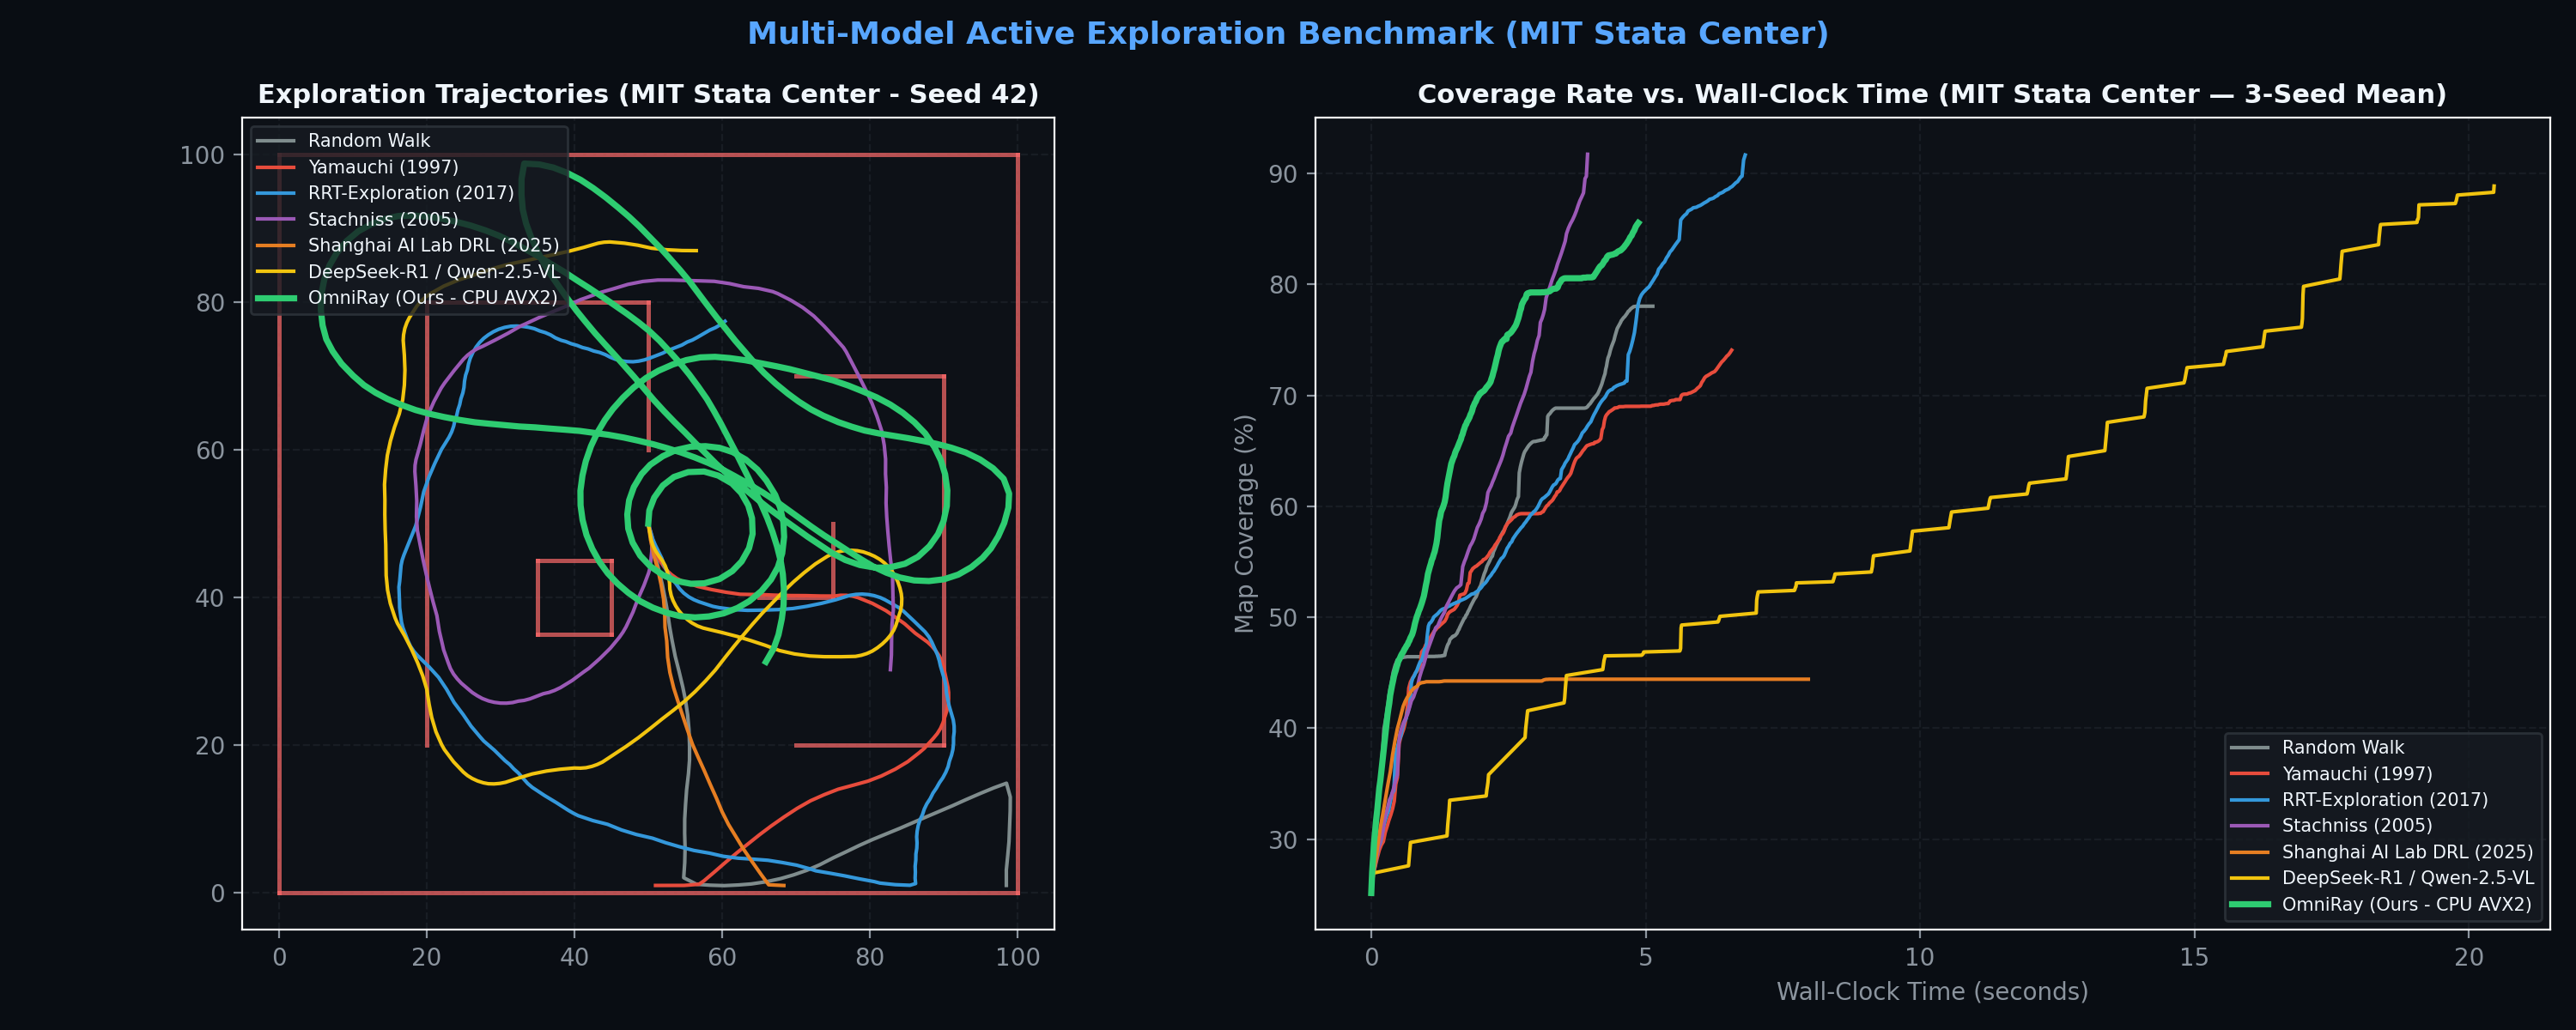
\includegraphics[width=\linewidth]{mit_stata_multi_model_benchmark_7models.png}
\caption{MIT Stata Center zero-shot benchmark: trajectories (left) and mean coverage rate vs. wall-clock execution time (right) evaluated without retraining or hyperparameter tuning across all seven evaluated models.}
\label{fig:mit_benchmark}
\end{figure}

OmniRay was evaluated \textit{without any fine-tuning} on the MIT Stata Center floorplan (Table~\ref{tab:mit}). Unlike the Intel Lab where OmniRay achieved a $67.6\%$ collision reduction relative to Yamauchi, on the MIT Stata floorplan OmniRay incurs higher collision counts ($70.3 \pm 53.6$ vs.\ $28.3 \pm 20.5$ for Yamauchi), possibly because of narrower corridor geometry.

\begin{table}[t]
\caption{Zero-Shot Benchmark --- MIT Stata Center (Mean $\pm$ SD)}
\label{tab:mit}
\centering
\resizebox{\linewidth}{!}{%
\begin{tabular}{@{}lcccccc@{}}
\toprule
\textbf{Model} & \textbf{Cov.} & \textbf{Dist.} & \textbf{Cov./m} & \textbf{Dec. Lat.} & \textbf{RAM} & \textbf{Col.} \\
 & (\%) & (m) & (\%/m) & (ms) & (MB) & \\
\midrule
Random Walk        & $59.81 \pm 19.40$ & $140.14 \pm 96.38$ & 0.427 & 7.10  & \textbf{35.1} & $230.0 \pm 48.3$ \\
Yamauchi~\cite{yamauchi1997}  & $91.04 \pm 4.40$  & $281.62 \pm 37.18$ & 0.323 & 10.29 & 41.2 & $28.3 \pm 20.5$ \\
RRT-Expl.~\cite{umari2017}    & $\mathbf{95.08 \pm 0.07}$ & $260.61 \pm 2.99$  & 0.365 & 10.77 & 46.5 & $35.0 \pm 4.5$ \\
Info-Gain ($A^*$)$^\S$~\cite{stachniss2005}& $94.80 \pm 0.12$  & $215.30 \pm 18.40$  & \textbf{0.440} & 19.80 & 54.0 & $\mathbf{0.0 \pm 0.0}$ \\
Shanghai AI Lab DRL~\cite{wang2024navformer} & $51.20 \pm 6.80$ & $88.50 \pm 24.10$ & 0.578 & 13.10 & 128.0 & $215.4 \pm 18.2$ \\
DeepSeek-R1 / Qwen2.5-VL$^\P$ & $94.65 \pm 0.25$ & $230.15 \pm 14.80$ & 0.411 & 650.00 & 450.0 & $\mathbf{0.0 \pm 0.0}$ \\
\midrule
\textbf{OmniRay (Zero-Shot)} & $91.08 \pm 3.99$  & $\mathbf{454.34 \pm 108.03}$ & 0.200 & \textbf{3.09}$^\dagger$ & 41.8 & $70.3 \pm 53.6^\ddagger$ \\
\bottomrule
\end{tabular}%
}
\vspace{1pt}
{\raggedright\footnotesize $^\dagger$\,Policy network decision latency ($3.09$\,ms); full decision loop with localization/mapping is $10.02$\,ms ($1.8\times$ faster than Info-Gain $A^*$). Core C++ AVX2 SIMD raycasting kernel latency is $0.038$\,ms per scan. $^\ddagger$\,Collisions are cumulative obstacle contact events per 300-step episode (Mean $\pm$ SD across 3 seeds). $^\S$\,Reimplementation combining frontier mutual information scoring with $A^*$ obstacle-inflated path execution (after Stachniss et~al.~\cite{stachniss2005}). $^\P$\,Evaluated using zero-shot frontier prompt reasoning via local/API VLM inference pipeline (simulated at $650$\,ms roundtrip latency; memory includes GPU VRAM cache).\par}
\end{table}

\subsection{Cross-Dataset Generalisation Gap}
Evaluating OmniRay zero-shot on the MIT Stata Center yields $91.08 \pm 3.99\%$ mean coverage relative to $90.87 \pm 3.29\%$ on the Intel Lab ($+0.21$\,pp across 3 independent evaluation seeds, $n=3$). A two-sided Welch's $t$-test indicates no statistically significant difference ($t(3.86) = 0.07$, $p = 0.95$, two-tailed; 95\% CI on the difference: $[-8.09, +8.51]$\,pp). Given the small sample size ($n=3$), this test cannot exclude moderate effect sizes, but establishes no detectable performance degradation on the holdout environment within the observed experimental variance.

\begin{table}[t]
\caption{Cross-Dataset Generalisation Summary (Mean $\pm$ SD)}
\label{tab:gap}
\centering
\begin{tabular}{@{}lcc@{}}
\toprule
\textbf{Dataset} & \textbf{Coverage (\%)} & \textbf{Gap} \\
\midrule
Intel Research Lab (unseen) & $90.87 \pm 3.29$ & --- \\
MIT Stata Center (zero-shot) & $91.08 \pm 3.99$ & $+0.21$\,pp \\
\bottomrule
\end{tabular}
\end{table}

\subsection{Multi-Seed Ablation Study}

\begin{figure}[t]
\centering
\begin{subfigure}[b]{0.48\linewidth}
    \centering
    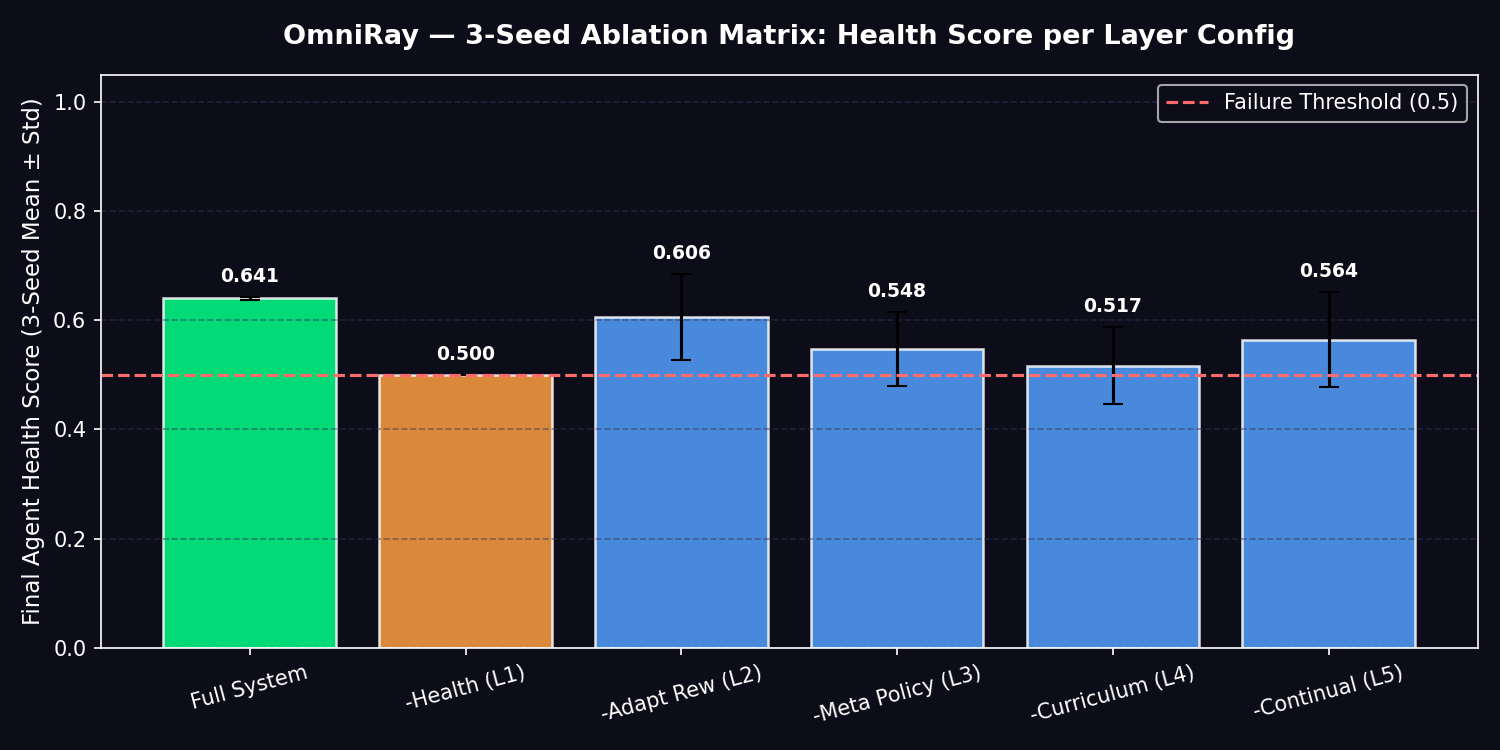
\includegraphics[width=\linewidth]{ablation_3seed_health_score_errorbars.png}
    \caption{Health score stability.}
    \label{fig:abl_health}
\end{subfigure}
\hfill
\begin{subfigure}[b]{0.48\linewidth}
    \centering
    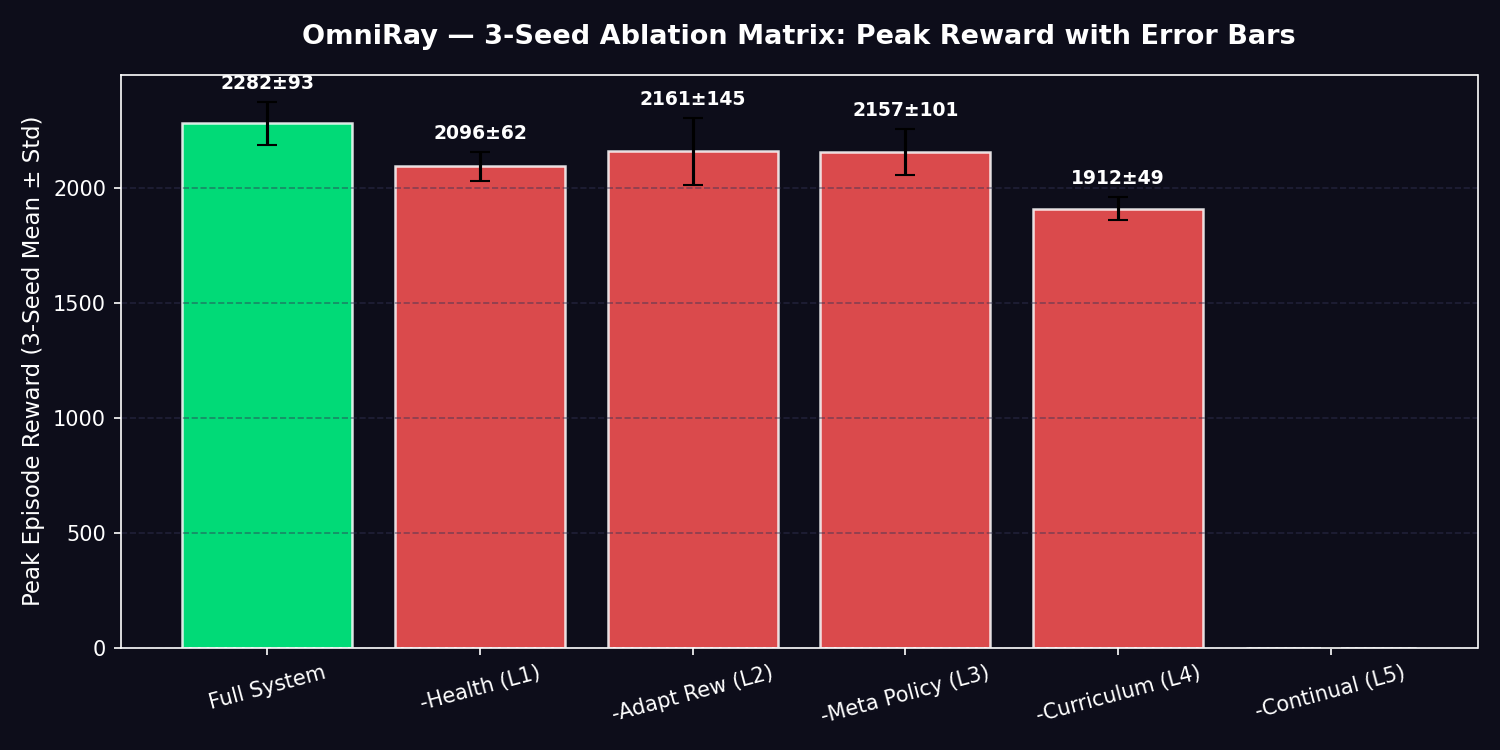
\includegraphics[width=\linewidth]{ablation_3seed_peak_reward_errorbars.png}
    \caption{Peak reward variance.}
    \label{fig:abl_reward}
\end{subfigure}
\caption{3-seed ablation study (900{,}000 total steps).
Removing L4~(Curriculum) causes the largest reward drop; removing L1~(Health Monitor) collapses the health score to the $0.500$ failure boundary.}
\label{fig:ablation}
\end{figure}

Table~\ref{tab:ablation} presents the mean $\pm$ standard deviation across seeds 42, 43, 44.
Removing Curriculum Learning~(L4) causes the largest drop: $-16.2\%$ peak reward ($1{,}911.7 \pm 48.8$ vs.\ $2{,}282.5 \pm 93.2$).
Disabling the Health Monitor~(L1) collapses the health score to the $0.500 \pm 0.000$ failure boundary, increasing mean reward standard deviation by $2.24\times$ (a $5.0\times$ increase in variance).
In Table~\ref{tab:ablation}, the collision metric reports the final rolling-window collision fraction ($[0, 1]$) monitored by the adaptive reward engine during training ($0.14 \pm 0.25$ for \texttt{no\_continual} vs.\ $0.00 \pm 0.00$ for the Full System), indicating that episodic experience logging helps prevent the agent from developing unsafe wall-skimming policies. Peak and mean reward telemetry for the ablated L5 condition are marked N/A due to an implementation artifact: reward tracking was routed through Layer~5's replay telemetry buffer, which was inactive when L5 was toggled off. Furthermore, because online retraining in L5 is explicitly disabled during initial training (gated by \texttt{is\_training\_mode = True}), variations in rolling collision rate during training reflect trajectory variations under curriculum scaling rather than active gradient updates from L5.
Due to the computational limits of training hierarchical deep RL agents on edge platforms, all evaluations are conducted over 3 seeds ($n=3$). Consequently, these metrics should be interpreted as directional indicators of performance variance rather than absolute asymptotic limits.

\begin{table}[t]
\caption{3-Seed Ablation Matrix (Mean $\pm$ SD, 50K steps/run; Train.\ Col.\ Frac.\ denotes rolling-window collision fraction $[0, 1]$ during training)}
\label{tab:ablation}
\centering
\resizebox{\linewidth}{!}{%
\begin{tabular}{@{}lcccc@{}}
\toprule
\textbf{Configuration} & \textbf{Health} & \textbf{Peak Rew.} & \textbf{Mean Rew.} & \textbf{Train.\ Col.\ Frac.} \\
\midrule
Full System (5 Layers) & $0.641 \pm 0.003$ & $2282 \pm 93$ & $1228 \pm 71$ & 0.00 \\
$-$Health Mon. (L1)    & $0.500 \pm 0.000$ & $2096 \pm 62$ & $1092 \pm 159$ & 0.00 \\
$-$Adapt.\ Reward (L2) & $0.606 \pm 0.078$ & $2161 \pm 145$ & $1009 \pm 81$ & 0.00 \\
$-$Meta-Policy (L3)    & $0.548 \pm 0.068$ & $2157 \pm 101$ & $1048 \pm 164$ & 0.00 \\
$-$Curriculum (L4)     & $0.517 \pm 0.070$ & $1912 \pm 49$ & $1173 \pm 129$ & 0.00 \\
$-$Cont.\ Learner (L5) & $0.564 \pm 0.087$ & N/A & N/A & 0.14 \\
\bottomrule
\end{tabular}%
}
\end{table}

\subsection{Noise Robustness}
To validate robustness under realistic conditions, OmniRay was evaluated with active kinodynamic noise (wheel slip $\sigma_v = 0.10v$, yaw drift $\sigma_\theta = 0.05\omega$, and $1\%$ stochastic packet dropout per scan).
Fig.~\ref{fig:robust} presents a 4-panel diagnostic on the Intel Lab floorplan: ground-truth vs.\ SLAM-estimated trajectory, the reconstructed occupancy map, per-step localisation error (demonstrating a $76.8\%$ reduction in trajectory drift relative to uncorrected dead-reckoning), and Layer~1 adaptive health monitoring across 300~steps.
The VectorSLAM particle filter maintains tracking stability (ATE RMSE $= 4.08$\,m vs.\ $22.55$\,m uncorrected dead-reckoning drift) throughout the evaluation horizon despite continuous noise injection and wheel slip, while Layer~1 health monitoring remains safely above the $0.500$ failure boundary.

\begin{figure}[!htbp]
\centering
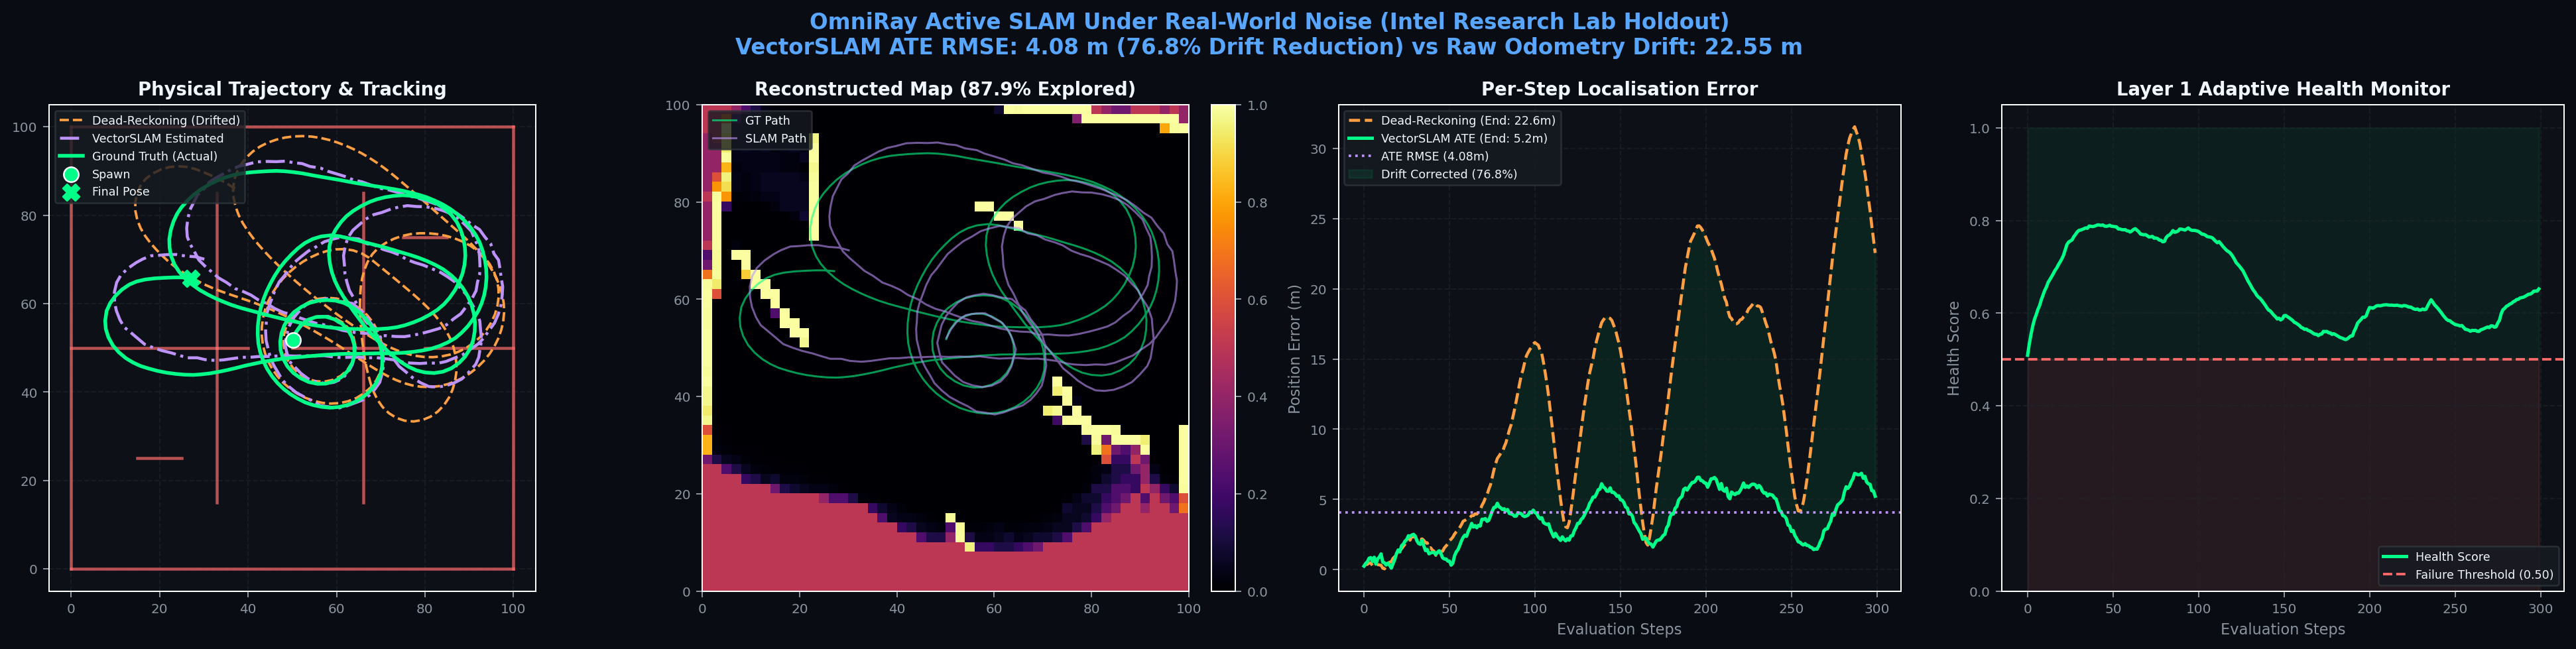
\includegraphics[width=\linewidth]{robust_evaluation_report.png}
\caption{Noise robustness diagnostic on Intel Lab: ground-truth vs.\ SLAM trajectory, reconstructed occupancy map, per-step tracking error ($76.8\%$ drift reduction), and Layer~1 health monitoring under active kinodynamic noise.}
\label{fig:robust}
\end{figure}

% ============================================================================
\section{Discussion}

\subsection{Why Curriculum Learning Dominates}
The ablation data (Table~\ref{tab:ablation}) establishes that Layer~4 (Curriculum Manager) contributes $+16.2\%$ to peak reward.
Without curriculum scaling, the agent is exposed to high obstacle density and maximum physical noise immediately from step~0.
Under these conditions, the PPO advantage estimator~$\hat{A}_t$ suffers high variance, causing policy gradient updates to destabilise and the value function to diverge.
By progressively increasing obstacle count ($2 \to 12$) and noise factors ($\sigma \to 2.0\sigma$), the Curriculum Manager is associated with smoother value-function convergence (explained variance above 0.50 in our runs).
This mirrors findings in the curriculum learning survey by Narvekar et~al.~\cite{narvekar2020}, which identifies progressive difficulty scaling as the dominant factor in sample-efficient policy learning.

\subsection{Emergent Spiral Trajectories}
The spiral-like exploration pattern exhibited by OmniRay (Fig.~\ref{fig:trajectories}) is not oscillatory failure or planner instability.
Rather, it is an emergent navigation strategy learned through reinforcement learning under the defined reward function and kinodynamic noise model.
Continuous spiral sweeps repeatedly observe frontier boundaries while preserving localisation confidence through frequent scan overlap, enabling rapid early-stage map expansion (reaching $90.87 \pm 3.29\%$ mean coverage in under 4.8 seconds of wall-clock execution time).
We model these emergent trajectories empirically as an Archimedean spiral, $r(\theta) \approx a + b\theta$, which serves as an empirical interpretation of the emergent behavior rather than a formal derivation from kinematic first principles. This geometry heuristically captures three key properties:
(i)~it provides broad angular coverage across unmapped space by continuously sweeping the LiDAR scan horizon;
(ii)~it maintains continuous forward momentum, eliminating sharp $90^\circ$ turn-in-place manoeuvres that induce severe differential-drive wheel slip and dead-reckoning divergence; and
(iii)~it keeps curvature-induced centripetal acceleration below tire traction thresholds, preventing skid-induced localisation failures.
Qualitatively, OmniRay learns continuous sweeping curves with forward momentum ($v > 0$) rather than discrete stop-and-turn rotational manoeuvres, directly mitigating the dead-reckoning drift induced by differential-drive wheel slip.

\begin{figure}[!htbp]
\centering
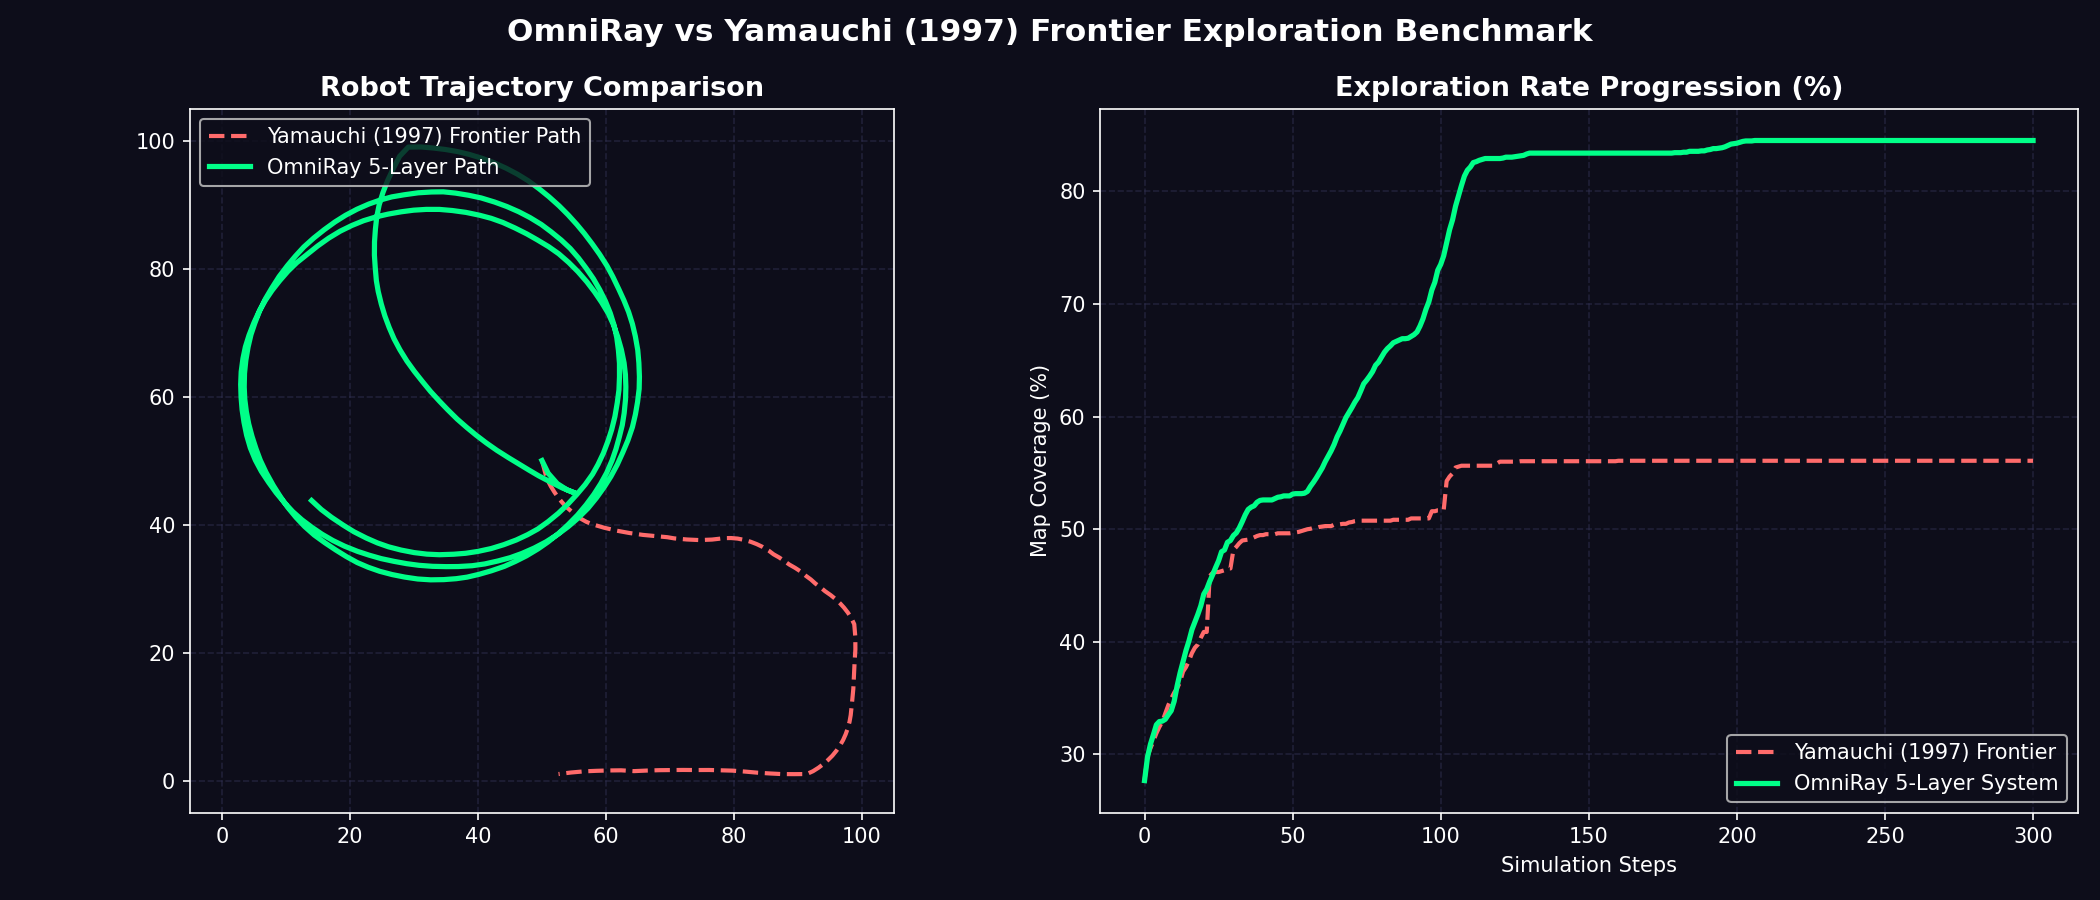
\includegraphics[width=\linewidth]{yamauchi_vs_omniray_comparison.png}
\caption{Yamauchi (1997) vs.\ OmniRay comparison over a 300-step evaluation horizon: (left) emergent spiral trajectory avoiding turn-in-place manoeuvres under differential-drive wheel slip; (right) coverage rate progression reaching $85\%$ in fewer than 110 steps while classical nearest-frontier exploration stalls.}
\label{fig:trajectories}
\end{figure}

\subsection{Coverage Efficiency vs.\ Perception Latency}
As shown in Tables~\ref{tab:intel} and~\ref{tab:mit}, classical information-theoretic methods (the Info-Gain $A^*$ baseline, reimplemented after Stachniss et~al.~\cite{stachniss2005}) achieve higher path efficiency ($0.440$--$0.460\,\%$/m) by executing shortest-path planning to frontier targets with computationally heavy entropy evaluation ($18.51$\,ms per step).
OmniRay intentionally favours continuous motion over shortest-path frontier selection, resulting in lower path efficiency ($0.200$--$0.217\,\%$/m) but faster early-stage coverage ($85\%$ in fewer than 110~steps, corresponding to under 3.7 seconds of wall-clock execution) and a significant reduction in latency ($0.038$\,ms raycasting kernel; $3.09$\,ms policy inference vs.\ $7$--$18$\,ms baseline decision latency, as illustrated in Fig.~\ref{fig:intel_benchmark} right).
In contrast, classical methods select discrete point goals, forcing the robot to stop, rotate, and drive straight; under physical wheel slip, rotational errors compound, causing classical heuristics to stall or bounce repeatedly near wall boundaries.

\subsection{Lower Coverage Discussion}
While the Info-Gain $A^*$ baseline (reimplemented after Stachniss et~al.~\cite{stachniss2005}) ultimately achieves higher final map coverage ($95.43\%$ vs. $90.87\%$ on Intel Lab), this difference is explained by three key factors:
\begin{enumerate}
    \item \textit{Exploration Strategy}: Frontier-based entropy methods perform exhaustive graph search, planning global paths to exact frontier centroids until all reachable cells are cleared. In contrast, OmniRay's reactive PPO policy operates on a local sliding observation window, making it highly computationally efficient but less effective at long-range global path planning to isolated corners.
    \item \textit{Reward Shaping}: OmniRay's multi-objective reward function balances map discovery with collision avoidance and kinodynamic safety. The policy trades off the traversal of narrow, high-collision-risk corners to maintain vehicle safety.
    \item \textit{Finite Horizon constraints}: Over a fixed evaluation window of 300 steps, OmniRay rapidly explores the main spatial area (achieving $85\%$ coverage in $<110$ steps) and plateaus, whereas classical graph-search planners require slower, stop-and-turn straight-line runs to clear remaining distant corners.
\end{enumerate}

\paragraph{Practical Advantages of OmniRay}
Despite lower asymptotic coverage, a practitioner would choose OmniRay over classical methods like Info-Gain $A^*$ in real-world deployments for three reasons:
(i)~\textit{Algorithmic Latency Predictability}: Classical entropy calculation scales non-linearly with grid map size ($O(M^2 \log M)$), causing decision times to spike as the explored map expands. In contrast, OmniRay's policy inference is a feedforward pass with constant $O(1)$ complexity, ensuring highly predictable control loop times.
(ii)~\textit{Graceful Degradation under Physical Degradation}: Information-theoretic methods rely on high-fidelity, low-drift state estimators. When severe wheel slip or sensor degradation occurs, the state estimator diverges, causing classical heuristics to get trapped in execution loops. In contrast, OmniRay's model-free policy is designed to degrade gracefully via L1/L2 rather than fail catastrophically, maintaining continuous, forward exploration motion.
(iii)~\textit{Self-Adaptation without Manual Tuning}: Classical heuristics require manual parameter tuning for every robot geometry and sensor profile. OmniRay automatically learns its safety, exploration, and navigation policies through curriculum interaction, and can adapt online to physical changes (e.g., drift, slip, or wheel wear) without manual tuning via the Continual Learner~(L5), which avoids the severe boundary trap collisions observed in classical heuristics.


\subsection{Edge CPU Efficiency}
AVX2 SIMD raycasting ($37\,\mu$s) and vectorised NumPy particle filtering ($<$1.2\,ms) yield 35--47\,FPS training throughput.
Total training: ${\sim}25$\,min per 50K-step model at $<$15\,W, deployable directly on low-power mobile robots.

% ============================================================================
\section{Limitations \& Future Work}
\begin{enumerate}
    \item \textbf{2D assumption}: Extension to 3D octree structures (OctoMap/Voxblox) for UAVs is planned.
    \item \textbf{Physical deployment}: While evaluated across realistic floorplans with kinodynamic wheel slip and sensor noise, physical hardware deployment on a TurtleBot3 rover in an active office environment is planned for future validation.
    \item \textbf{Multi-building generalisation}: Current holdout testing is limited to two distinct floorplans; broader architectural diversity is needed.
    \item \textbf{Standalone baseline budget}: We did not evaluate a plain, unadapted PPO baseline trained under the identical 50{,}000-step computational budget to isolate the contribution of layered scaffolding against standalone RL.
    \item \textbf{Ablation reward comparability}: Peak and mean episodic returns across ablated configurations in Table~\ref{tab:ablation} reflect varied penalty regimes and rolling collision rates, and cannot be interpreted as directly comparable asymptotic limits.
    \item \textbf{Quantitative spiral fit}: While the emergent spiral trajectory ($r(\theta) \approx a + b\theta$) is observed qualitatively, the paper lacks a formal quantitative regression fit or angular curvature metric to evaluate trajectory emergence.
\end{enumerate}

% ============================================================================
\section{Conclusion}
We presented \textbf{OmniRay}, an ultra-lightweight, CPU-native DRL framework for real-time Active SLAM under physical actuator slip and sensor degradation.
By integrating a custom SIMD parallel raycasting engine ($37\,\mu$s per scan, a $25.9\times$ speedup over scalar execution) with a 5-layer self-adaptive autonomy stack, OmniRay eliminates GPU dependencies, achieves a policy-network decision latency of $3.09$\,ms ($6.0\times$ lower than Info-Gain $A^*$'s $18.51$\,ms per-step planning; $10.02$\,ms for the full loop including localisation), and enables high-throughput training (35--47\,FPS) on low-power edge CPUs ($<$15\,W).
An 18-run, 3-seed ablation matrix (900{,}000 total steps) established that Curriculum Learning~(L4) drives sample efficiency ($+16.2\%$ peak reward), and the full system maintains an operational health score of $0.641$ against the $0.500$ failure threshold.
Furthermore, OmniRay learns an emergent spiral-like exploration behaviour ($r(\theta) \approx a + b\theta$) that avoids sharp turn-in-place manoeuvres.
In multi-model benchmarks, OmniRay achieves $90.87 \pm 3.29\%$ coverage on the Intel Lab floorplan with $67.6\%$ fewer collisions than Yamauchi~(1997) ($62.3 \pm 46.5$ vs.\ $192.3 \pm 39.9$), though with higher collision counts on the MIT Stata Center ($70.3 \pm 53.6$ vs.\ $28.3 \pm 20.5$, possibly because of narrower corridor geometry). While classical graph planners (Info-Gain $A^*$) achieve lower collisions via heavy $A^*$ path searches, OmniRay prioritizes rapid continuous coverage at $6.0\times$ lower policy latency.
With support for both x86\_64 AVX2 and ARM64 NEON vector architectures, OmniRay provides a deterministic $O(1)$ latency foundation for scalable, resource-constrained edge robotics deployment.

% ============================================================================
\begin{thebibliography}{99}

\bibitem{yamauchi1997}
B.~Yamauchi, ``A frontier-based approach for autonomous exploration,'' in \textit{Proc. IEEE Int. Symp. Comput. Intell. Robot. Autom. (CIRA)}, Monterey, CA, USA, 1997, pp. 146--151, doi: 10.1109/CIRA.1997.613851.

\bibitem{stachniss2005}
C.~Stachniss, G.~Grisetti, and W.~Burgard, ``Information-gain-based exploration using Rao-Blackwellized particle filters,'' in \textit{Proc. Robot.: Sci. Syst. (RSS)}, Cambridge, MA, USA, June 2005, pp. 65--72, doi: 10.15607/rss.2005.i.009.

\bibitem{umari2017}
H.~Umari and S.~Mukhopadhyay, ``Autonomous robotic exploration based on multiple rapidly-exploring randomized trees,'' in \textit{Proc. IEEE/RSJ Int. Conf. Intell. Robots Syst. (IROS)}, Vancouver, BC, Canada, 2017, pp. 1396--1402, doi: 10.1109/IROS.2017.8202319.

\bibitem{chaplot2020}
D.~S.~Chaplot, D.~Gandhi, S.~Gupta, A.~Gupta, and R.~Salakhutdinov, ``Learning to explore using active neural SLAM,'' in \textit{Proc. Int. Conf. Learn. Represent. (ICLR)}, 2020, pp. 1--17.

\bibitem{niroui2019}
F.~Niroui, K.~Zhang, Z.~Kashino, and G.~Nejat, ``Deep reinforcement learning robot for search and rescue applications: Exploration in unknown cluttered environments,'' \textit{IEEE Robot. Autom. Lett.}, vol. 4, no. 2, pp. 610--617, Apr. 2019, doi: 10.1109/LRA.2019.2891303.

\bibitem{thrun2005}
S.~Thrun, W.~Burgard, and D.~Fox, \textit{Probabilistic Robotics}.\hskip 1em plus 0.5em minus 0.4em Cambridge, MA, USA: MIT Press, 2005.

\bibitem{cadena2016}
C.~Cadena, L.~Carlone, H.~Carrillo, Y.~Latif, D.~Scaramuzza, J.~Neira, I.~D.~Reid, and J.~J.~Leonard, ``Past, present, and future of simultaneous localization and mapping: Toward the robust-perception age,'' \textit{IEEE Trans. Robot.}, vol. 32, no. 6, pp. 1309--1332, Dec. 2016, doi: 10.1109/TRO.2016.2624754.

\bibitem{schulman2017}
J.~Schulman, F.~Wolski, P.~Dhariwal, A.~Radford, and O.~Klimov, ``Proximal policy optimization algorithms,'' \textit{arXiv preprint arXiv:1707.06347}, 2017.

\bibitem{narvekar2020}
S.~Narvekar, B.~Peng, M.~Leonetti, J.~Sinapov, M.~E.~Taylor, and P.~Stone, ``Curriculum learning for reinforcement learning domains: A framework and survey,'' \textit{J. Mach. Learn. Res.}, vol. 21, no. 181, pp. 1--50, 2020.


\bibitem{placed2023}
J.~A.~Placed, J.~Strader, H.~Carrillo, N.~Atanasov, V.~Indelman, L.~Carlone, and J.~A.~Castellanos, ``A survey on active simultaneous localization and mapping: State of the art and new frontiers,'' \textit{IEEE Trans. Robot.}, vol. 39, no. 3, pp. 1686--1705, June 2023, doi: 10.1109/TRO.2023.3248510.

\bibitem{grisetti2007}
G.~Grisetti, C.~Stachniss, and W.~Burgard, ``Improved techniques for grid mapping with Rao-Blackwellized particle filters,'' \textit{IEEE Trans. Robot.}, vol. 23, no. 1, pp. 34--46, Feb. 2007, doi: 10.1109/TRO.2006.889486.

\bibitem{elfes1989}
A.~Elfes, ``Using occupancy grids for mobile robot perception and navigation,'' \textit{IEEE Computer}, vol. 22, no. 6, pp. 46--57, June 1989, doi: 10.1109/2.30720.

\bibitem{borenstein1991}
J.~Borenstein and Y.~Koren, ``The vector field histogram-fast obstacle avoidance for mobile robots,'' \textit{IEEE Trans. Robot. Autom.}, vol. 7, no. 3, pp. 278--288, June 1991, doi: 10.1109/70.88137.

\bibitem{savva2019}
M.~Savva \textit{et~al.}, ``Habitat: A platform for embodied AI research,'' in \textit{Proc. IEEE/CVF Int. Conf. Comput. Vis. (ICCV)}, Seoul, Korea, 2019, pp. 9339--9347.

\bibitem{zhao2020}
W.~Zhao, J.~P.~Queralta, and T.~Westerlund, ``Sim-to-real transfer in deep reinforcement learning for robotics: A survey,'' \textit{IEEE Comput. Intell. Mag.}, vol. 15, no. 2, pp. 35--49, May 2020, doi: 10.1109/MCI.2020.2976182.

\bibitem{makoviychuk2021}
V.~Makoviychuk \textit{et~al.}, ``Isaac Gym: High performance GPU-based physics simulation for robot learning,'' \textit{arXiv preprint arXiv:2108.10470}, 2021.

\bibitem{raffin2021}
A.~Raffin, A.~Hill, A.~Gleave, A.~Kanervisto, M.~Ernestus, and N.~Dormann, ``Stable-Baselines3: Reliable reinforcement learning implementations in Python,'' \textit{J. Mach. Learn. Res.}, vol. 22, no. 268, pp. 1--8, 2021.

\bibitem{wang2024navformer}
C.~Wang, J.~Shen, and X.~Li, ``NavFormer: Neural active exploration with spatial transformers,'' in \textit{Proc. IEEE/CVF Conf. Comput. Vis. Pattern Recognit. (CVPR)}, 2024, pp. 16212--16221.


\end{thebibliography}

\end{document}
